
%% bare_conf.tex
%% V1.4
%% 2012/12/27
%% by Michael Shell
%% See:
%% http://www.michaelshell.org/
%% for current contact information.
%%
%% This is a skeleton file demonstrating the use of IEEEtran.cls
%% (requires IEEEtran.cls version 1.8 or later) with an IEEE conference paper.
%%
%% Support sites:
%% http://www.michaelshell.org/tex/ieeetran/
%% http://www.ctan.org/tex-archive/macros/latex/contrib/IEEEtran/
%% and
%% http://www.ieee.org/

%%*************************************************************************
%% Legal Notice:
%% This code is offered as-is without any warranty either expressed or
%% implied; without even the implied warranty of MERCHANTABILITY or
%% FITNESS FOR A PARTICULAR PURPOSE! 
%% User assumes all risk.
%% In no event shall IEEE or any contributor to this code be liable for
%% any damages or losses, including, but not limited to, incidental,
%% consequential, or any other damages, resulting from the use or misuse
%% of any information contained here.
%%
%% All comments are the opinions of their respective authors and are not
%% necessarily endorsed by the IEEE.
%%
%% This work is distributed under the LaTeX Project Public License (LPPL)
%% ( http://www.latex-project.org/ ) version 1.3, and may be freely used,
%% distributed and modified. A copy of the LPPL, version 1.3, is included
%% in the base LaTeX documentation of all distributions of LaTeX released
%% 2003/12/01 or later.
%% Retain all contribution notices and credits.
%% ** Modified files should be clearly indicated as such, including  **
%% ** renaming them and changing author support contact information. **
%%
%% File list of work: IEEEtran.cls, IEEEtran_HOWTO.pdf, bare_adv.tex,
%%                    bare_conf.tex, bare_jrnl.tex, bare_jrnl_compsoc.tex,
%%                    bare_jrnl_transmag.tex
%%*************************************************************************

% *** Authors should verify (and, if needed, correct) their LaTeX system  ***
% *** with the testflow diagnostic prior to trusting their LaTeX platform ***
% *** with production work. IEEE's font choices can trigger bugs that do  ***
% *** not appear when using other class files.                            ***
% The testflow support page is at:
% http://www.michaelshell.org/tex/testflow/



% Note that the a4paper option is mainly intended so that authors in
% countries using A4 can easily print to A4 and see how their papers will
% look in print - the typesetting of the document will not typically be
% affected with changes in paper size (but the bottom and side margins will).
% Use the testflow package mentioned above to verify correct handling of
% both paper sizes by the user's LaTeX system.
%
% Also note that the "draftcls" or "draftclsnofoot", not "draft", option
% should be used if it is desired that the figures are to be displayed in
% draft mode.
%
\documentclass[conference]{IEEEtran}
% Add the compsoc option for Computer Society conferences.
%
% If IEEEtran.cls has not been installed into the LaTeX system files,
% manually specify the path to it like:
% \documentclass[conference]{../sty/IEEEtran}





% Some very useful LaTeX packages include:
% (uncomment the ones you want to load)


% *** MISC UTILITY PACKAGES ***
%
%\usepackage{ifpdf}
% Heiko Oberdiek's ifpdf.sty is very useful if you need conditional
% compilation based on whether the output is pdf or dvi.
% usage:
% \ifpdf
%   % pdf code
% \else
%   % dvi code
% \fi
% The latest version of ifpdf.sty can be obtained from:
% http://www.ctan.org/tex-archive/macros/latex/contrib/oberdiek/
% Also, note that IEEEtran.cls V1.7 and later provides a builtin
% \ifCLASSINFOpdf conditional that works the same way.
% When switching from latex to pdflatex and vice-versa, the compiler may
% have to be run twice to clear warning/error messages.






% *** CITATION PACKAGES ***
%
%\usepackage{cite}
% cite.sty was written by Donald Arseneau
% V1.6 and later of IEEEtran pre-defines the format of the cite.sty package
% \cite{} output to follow that of IEEE. Loading the cite package will
% result in citation numbers being automatically sorted and properly
% "compressed/ranged". e.g., [1], [9], [2], [7], [5], [6] without using
% cite.sty will become [1], [2], [5]--[7], [9] using cite.sty. cite.sty's
% \cite will automatically add leading space, if needed. Use cite.sty's
% noadjust option (cite.sty V3.8 and later) if you want to turn this off
% such as if a citation ever needs to be enclosed in parenthesis.
% cite.sty is already installed on most LaTeX systems. Be sure and use
% version 4.0 (2003-05-27) and later if using hyperref.sty. cite.sty does
% not currently provide for hyperlinked citations.
% The latest version can be obtained at:
% http://www.ctan.org/tex-archive/macros/latex/contrib/cite/
% The documentation is contained in the cite.sty file itself.






% *** GRAPHICS RELATED PACKAGES ***
%
\ifCLASSINFOpdf
  % \usepackage[pdftex]{graphicx}
  % declare the path(s) where your graphic files are
  % \graphicspath{{../pdf/}{../jpeg/}}
  % and their extensions so you won't have to specify these with
  % every instance of \includegraphics
  % \DeclareGraphicsExtensions{.pdf,.jpeg,.png}
\else
  % or other class option (dvipsone, dvipdf, if not using dvips). graphicx
  % will default to the driver specified in the system graphics.cfg if no
  % driver is specified.
  % \usepackage[dvips]{graphicx}
  % declare the path(s) where your graphic files are
  % \graphicspath{{../eps/}}
  % and their extensions so you won't have to specify these with
  % every instance of \includegraphics
  % \DeclareGraphicsExtensions{.eps}
\fi
% graphicx was written by David Carlisle and Sebastian Rahtz. It is
% required if you want graphics, photos, etc. graphicx.sty is already
% installed on most LaTeX systems. The latest version and documentation
% can be obtained at: 
% http://www.ctan.org/tex-archive/macros/latex/required/graphics/
% Another good source of documentation is "Using Imported Graphics in
% LaTeX2e" by Keith Reckdahl which can be found at:
% http://www.ctan.org/tex-archive/info/epslatex/
%
% latex, and pdflatex in dvi mode, support graphics in encapsulated
% postscript (.eps) format. pdflatex in pdf mode supports graphics
% in .pdf, .jpeg, .png and .mps (metapost) formats. Users should ensure
% that all non-photo figures use a vector format (.eps, .pdf, .mps) and
% not a bitmapped formats (.jpeg, .png). IEEE frowns on bitmapped formats
% which can result in "jaggedy"/blurry rendering of lines and letters as
% well as large increases in file sizes.
%
% You can find documentation about the pdfTeX application at:
% http://www.tug.org/applications/pdftex





% *** MATH PACKAGES ***
%
%\usepackage[cmex10]{amsmath}
% A popular package from the American Mathematical Society that provides
% many useful and powerful commands for dealing with mathematics. If using
% it, be sure to load this package with the cmex10 option to ensure that
% only type 1 fonts will utilized at all point sizes. Without this option,
% it is possible that some math symbols, particularly those within
% footnotes, will be rendered in bitmap form which will result in a
% document that can not be IEEE Xplore compliant!
%
% Also, note that the amsmath package sets \interdisplaylinepenalty to 10000
% thus preventing page breaks from occurring within multiline equations. Use:
%\interdisplaylinepenalty=2500
% after loading amsmath to restore such page breaks as IEEEtran.cls normally
% does. amsmath.sty is already installed on most LaTeX systems. The latest
% version and documentation can be obtained at:
% http://www.ctan.org/tex-archive/macros/latex/required/amslatex/math/





% *** SPECIALIZED LIST PACKAGES ***
%
%\usepackage{algorithmic}
% algorithmic.sty was written by Peter Williams and Rogerio Brito.
% This package provides an algorithmic environment fo describing algorithms.
% You can use the algorithmic environment in-text or within a figure
% environment to provide for a floating algorithm. Do NOT use the algorithm
% floating environment provided by algorithm.sty (by the same authors) or
% algorithm2e.sty (by Christophe Fiorio) as IEEE does not use dedicated
% algorithm float types and packages that provide these will not provide
% correct IEEE style captions. The latest version and documentation of
% algorithmic.sty can be obtained at:
% http://www.ctan.org/tex-archive/macros/latex/contrib/algorithms/
% There is also a support site at:
% http://algorithms.berlios.de/index.html
% Also of interest may be the (relatively newer and more customizable)
% algorithmicx.sty package by Szasz Janos:
% http://www.ctan.org/tex-archive/macros/latex/contrib/algorithmicx/




% *** ALIGNMENT PACKAGES ***
%
%\usepackage{array}
% Frank Mittelbach's and David Carlisle's array.sty patches and improves
% the standard LaTeX2e array and tabular environments to provide better
% appearance and additional user controls. As the default LaTeX2e table
% generation code is lacking to the point of almost being broken with
% respect to the quality of the end results, all users are strongly
% advised to use an enhanced (at the very least that provided by array.sty)
% set of table tools. array.sty is already installed on most systems. The
% latest version and documentation can be obtained at:
% http://www.ctan.org/tex-archive/macros/latex/required/tools/


% IEEEtran contains the IEEEeqnarray family of commands that can be used to
% generate multiline equations as well as matrices, tables, etc., of high
% quality.




% *** SUBFIGURE PACKAGES ***
%\ifCLASSOPTIONcompsoc
%  \usepackage[caption=false,font=normalsize,labelfont=sf,textfont=sf]{subfig}
%\else
%  \usepackage[caption=false,font=footnotesize]{subfig}
%\fi
% subfig.sty, written by Steven Douglas Cochran, is the modern replacement
% for subfigure.sty, the latter of which is no longer maintained and is
% incompatible with some LaTeX packages including fixltx2e. However,
% subfig.sty requires and automatically loads Axel Sommerfeldt's caption.sty
% which will override IEEEtran.cls' handling of captions and this will result
% in non-IEEE style figure/table captions. To prevent this problem, be sure
% and invoke subfig.sty's "caption=false" package option (available since
% subfig.sty version 1.3, 2005/06/28) as this is will preserve IEEEtran.cls
% handling of captions.
% Note that the Computer Society format requires a larger sans serif font
% than the serif footnote size font used in traditional IEEE formatting
% and thus the need to invoke different subfig.sty package options depending
% on whether compsoc mode has been enabled.
%
% The latest version and documentation of subfig.sty can be obtained at:
% http://www.ctan.org/tex-archive/macros/latex/contrib/subfig/




% *** FLOAT PACKAGES ***
%
%\usepackage{fixltx2e}
% fixltx2e, the successor to the earlier fix2col.sty, was written by
% Frank Mittelbach and David Carlisle. This package corrects a few problems
% in the LaTeX2e kernel, the most notable of which is that in current
% LaTeX2e releases, the ordering of single and double column floats is not
% guaranteed to be preserved. Thus, an unpatched LaTeX2e can allow a
% single column figure to be placed prior to an earlier double column
% figure. The latest version and documentation can be found at:
% http://www.ctan.org/tex-archive/macros/latex/base/


%\usepackage{stfloats}
% stfloats.sty was written by Sigitas Tolusis. This package gives LaTeX2e
% the ability to do double column floats at the bottom of the page as well
% as the top. (e.g., "\begin{figure*}[!b]" is not normally possible in
% LaTeX2e). It also provides a command:
%\fnbelowfloat
% to enable the placement of footnotes below bottom floats (the standard
% LaTeX2e kernel puts them above bottom floats). This is an invasive package
% which rewrites many portions of the LaTeX2e float routines. It may not work
% with other packages that modify the LaTeX2e float routines. The latest
% version and documentation can be obtained at:
% http://www.ctan.org/tex-archive/macros/latex/contrib/sttools/
% Do not use the stfloats baselinefloat ability as IEEE does not allow
% \baselineskip to stretch. Authors submitting work to the IEEE should note
% that IEEE rarely uses double column equations and that authors should try
% to avoid such use. Do not be tempted to use the cuted.sty or midfloat.sty
% packages (also by Sigitas Tolusis) as IEEE does not format its papers in
% such ways.
% Do not attempt to use stfloats with fixltx2e as they are incompatible.
% Instead, use Morten Hogholm'a dblfloatfix which combines the features
% of both fixltx2e and stfloats:
%
% \usepackage{dblfloatfix}
% The latest version can be found at:
% http://www.ctan.org/tex-archive/macros/latex/contrib/dblfloatfix/




% *** PDF, URL AND HYPERLINK PACKAGES ***
%
%\usepackage{url}
% url.sty was written by Donald Arseneau. It provides better support for
% handling and breaking URLs. url.sty is already installed on most LaTeX
% systems. The latest version and documentation can be obtained at:
% http://www.ctan.org/tex-archive/macros/latex/contrib/url/
% Basically, \url{my_url_here}.

%*** para suportar acentuação ***
\usepackage[utf8]{inputenc}

%*** para suportar tabelas com colunas mergeadas ***
\usepackage{multirow}

%*** Para inclusão de imagens e permitir rotacionar texto ***
\usepackage{graphicx}			% Inclusão de gráficos
\graphicspath{ {./} }			% localizando as imagens

%*** Para ajustar a largura das colunas e para multilinhas nas células ***
\usepackage{array}
\newcolumntype{L}{>{\centering\arraybackslash}m{0,75cm}}
\newcolumntype{M}{>{\centering\arraybackslash}m{3cm}}

% *** Do not adjust lengths that control margins, column widths, etc. ***
% *** Do not use packages that alter fonts (such as pslatex).         ***
% There should be no need to do such things with IEEEtran.cls V1.6 and later.
% (Unless specifically asked to do so by the journal or conference you plan
% to submit to, of course. )


% correct bad hyphenation here
\hyphenation{op-tical net-works semi-conduc-tor}


\begin{document}
%
% paper title
% can use linebreaks \\ within to get better formatting as desired
% Do not put math or special symbols in the title.
\title{Coletando dados de memória de uma máquina em nuvem para análise forense}


% author names and affiliations
% use a multiple column layout for up to three different
% affiliations
\author{\IEEEauthorblockN{Hamilton Fonte II}
\IEEEauthorblockA{Universidade de São Paulo (USP)\\
Escola Politécnica - Engenharia de Computação\\
Programa de Pós Graduação em Engenharia Elétrica\\
São Paulo, SP, Brasil\\
Email: hamiltonii@gmail.com}
\and
\IEEEauthorblockN{Marcus Simplício Jr.}
\IEEEauthorblockA{Orientador \\
Universidade de São Paulo (USP)\\
Escola Politécnica - Engenharia de Computação\\
Programa de Pós Graduação em Engenharia Elétrica\\
São Paulo, SP, Brasil}
}

% conference papers do not typically use \thanks and this command
% is locked out in conference mode. If really needed, such as for
% the acknowledgment of grants, issue a \IEEEoverridecommandlockouts
% after \documentclass

% for over three affiliations, or if they all won't fit within the width
% of the page, use this alternative format:
% 
%\author{\IEEEauthorblockN{Michael Shell\IEEEauthorrefmark{1},
%Homer Simpson\IEEEauthorrefmark{2},
%James Kirk\IEEEauthorrefmark{3}, 
%Montgomery Scott\IEEEauthorrefmark{3} and
%Eldon Tyrell\IEEEauthorrefmark{4}}
%\IEEEauthorblockA{\IEEEauthorrefmark{1}School of Electrical and Computer Engineering\\
%Georgia Institute of Technology,
%Atlanta, Georgia 30332--0250\\ Email: see http://www.michaelshell.org/contact.html}
%\IEEEauthorblockA{\IEEEauthorrefmark{2}Twentieth Century Fox, Springfield, USA\\
%Email: homer@thesimpsons.com}
%\IEEEauthorblockA{\IEEEauthorrefmark{3}Starfleet Academy, San Francisco, California 96678-2391\\
%Telephone: (800) 555--1212, Fax: (888) 555--1212}
%\IEEEauthorblockA{\IEEEauthorrefmark{4}Tyrell Inc., 123 Replicant Street, Los Angeles, California 90210--4321}}




% use for special paper notices
%\IEEEspecialpapernotice{(Invited Paper)}




% make the title area
\maketitle

% As a general rule, do not put math, special symbols or citations
% in the abstract
\begin{abstract}
A adoção de arquiteturas em nuvem aumenta a cada dia e com ele também os casos de uso dessas arquiteturas para fins ilícitos. Por sua natureza volátil, coletar evidências
para análise forense neste ambiente tem esbarrado em desafios práticos e legais. Este trabalho analisa as soluções propostas para resolver os principais problemas isolados
e propõe uma solução fim a fim para a coleta de evidências em núvem. A pesquisa é focada na reprodutibilidade do processo de coleta e na garantia de custódia da evidência
onde propomos uma forma de relacionar a evidência a sua origem virtual, transportar e armazenar mantendo sua credibilidade.
\end{abstract}

% no keywords




% For peer review papers, you can put extra information on the cover
% page as needed:
% \ifCLASSOPTIONpeerreview
% \begin{center} \bfseries EDICS Category: 3-BBND \end{center}
% \fi
%
% For peerreview papers, this IEEEtran command inserts a page break and
% creates the second title. It will be ignored for other modes.
\IEEEpeerreviewmaketitle



\section{Introdução}
Aumento do uso de soluções de virtualização e a implementação de arquiteturas em nuvem que escalam automáticamente \cite{Amazon2016} trouxe a questão da volatilidade 
das máquinas virtuais. Uma aplicação hospedada na nuvem sob um pico de uso e configurada para tal, pode clonar máquinas e adiciona-las ao grupo para atender a demanda. 
Passado este pico, as máquinas que foram clonadas são despejadas, seus recursos liberados e o conjunto retorna ao tamanho inicial. Com as ameaças que atuam diretamente 
na memória sem deixar rastros no disco da máquina afetada, se estas forem usadas para algum evento ilícito, as evidências do acontecimento contidas nelas 
serão para sempre perdidas.

Do ponto de vista forense, praticantes e pesquisadores concordam que aspectos de multi-inquilino e multi-jurisdição próprios soluções em nuvem figuram entre as principais 
dificuldades para coleta de evidência \cite{Bash2015a}. O aspecto multi-inquilino impede a remoção do hardware pois como ele é compartilhado com vários usuários, 
removê-los seria uma violação de privacidade de usuários não relacionados a investigação. Por fim a característica distribuída pode alocar informação relevante a 
investigação em vários países dificultando por razões jurídicas a obtenção da mesma \cite{Dykstra2012a} pois não é garantida a cooperação de instituições de outros países a investigações
em curso além de suas fronteiras.

Para o escopo deste trabalho estamos considerando 4 tipos de ataques realizados diretamente na memória e que não deixam rastros no disco da máquina, todos baseados 
em injeção de código \cite{Case2014}.

\begin{itemize}
 \item \textbf{Injeção remota de bibliotecas} - Um processo malicioso força o processo alvo a carregar uma biblioteca em seu espaço de memória. Uma vez carregada seus símbolos
 podem ser resolvidos pelo processo de resolução do sistema operacional e tem os mesmos privilégios do executável em que ela foi injetada. A biblioteca existe fisicamente em 
 alguma localização remota. Este processo de infecção é usado para o deployment de worms e rootkits. Uma estratégia usada é a de espalhar a biblioteca em vários processos
 de uma mesma máquina dificultando sua desinfecção \cite{Miller2004}.
 \item \textbf{Injeção remota de código} - Um processo malicioso escreve código como uma sequência de bytes diretamente no espaço de memória de um processo alvo e força este 
 último a executa-lo. O código pode por exemplo ser um script de shell
 \item \textbf{Injeção reflexiva de biblioteca} - Um processo malicioso escreve diretamente na memória de um processo alvo, como uma sequência de bytes, o código de uma biblioteca
 e força o processo alvo a executa-la. Nesta forma de ataque a biblioteca não existe fisicamente, é o método preferido de injeção de código uma vez que seu carregamento não
 é registrado no sistema operacional tornando-o assim, mais difícil de detectar \cite{Fewer2008}.
 \item \textbf{Injeção de processo vazio} - Um processo malicioso dispara uma instância de um processo legítimo no estado suspenso, a área do executável é liberada e realocada com 
 código malicioso.
\end{itemize}

Este documento esta organizado da seguinte forma: Na seção II falamos brevemente sobre soluções em nuvem, na seção III falamos sobre a evolução da forense e os desafios
que as soluções em nuvem trouxeram para a forense, na seção IV analisamos os trabalhos na área de forense de memória, na seção V descrevemos a solução proposta para 
resolver os problemas descritos em III, na VI expomos nossas conclusões e na VII elencamos os trabalhos futuros.

\section{Adoção de arquiteturas em nuvem}

A nuvem é um sistema em que recursos computacionais são oferecidos como serviço onde os usuários são cobrados pelo seu uso. A infra-estrutura é composta de máquinas fisicas
contendo cada uma um número variável de máquinas virtuais que implementam este serviço \cite{Sousa2009}. Há três modelos de comercialização de uso da nuvem, plataforma como serviço (PAAS), 
software como serviço(SAAS) e pertinente e este trabalho Infraestrutura como serviço (IAAS). O uso de soluções baseadas em nuvem tem crescido muito ultimamente, de janeiro 
de 2016 a maio de 2016 mais de 1000 bases de dados foram migradas para a AWS. \cite{Amazon2016}.

Uma forma mais recente de arquitetura em nuvem introduzida em 2008, os Containers Linux (LXC), proveram uma série de ferramentas para tirar vantagens das funcionalidades 
de cgroups e namespacing do kernel do Linux. Este conceito foi evoluindo e várias soluções de containerização sugiram como IMCTFY, Rocket e Docker. Container é uma forma 
de isolamento entre processos onde os containers partilham o mesmo kernel e tem sido usado para desenvolver serviços baseado em vitualização. A adoção de container tem 
crescido muito, segundo o "Container Market Adoption Survey 2016", das 235 empresas que responderam o survey 76\% delas utilizam containers em ambiente de produção.

\section{Forense de memória em nuvem}

A evolução da forense digital pode ser descrita em 3 fases \cite{Charters2008} A primeira ad-hoc se caracteriza pela falta de estrutura, processos, ferramental e 
objetivos. Nesta fase evidências apresentadas em processos legais eram descartadas com base em erros procedurais e falta de garantias de acurácia ou cadeia de custódia. 
Foi nesta fase que acusados de crimes usando um computador eram soltos sob justificativa de terem tido sua privacidade violada pelos investigadores. 
Na segunda fase começa a estruturação da forense, surgem as primeiras políticas e processos de coleta, armazenamento, transpórte e análise da evidência. O primeiro
processo proposto por Palmer G. em 2001 na primeira Digital Forensics Research Conference ficou conhecido como DIP, o próprio Palmer julgava o modelo incompleto. Em 2002 
Reith M. propôs o Abstract Digital Forensics Model que adicionava ao DIP estágios que faltava a este. Em 2003 Carrier e Spafford propuseram o Integrated Digital Investigation 
Process. Baseado nas técnicas e teorias da forense física e finalmente em 2004 Baryamureeba e Tushabe propuseram o Enhanced Digital Investigation Process Model, uma evolução
de Carrier e Spafford. Importante notar que esses modelos foram todos propostos antes que a forma atual de computação em nuvem estivesse disponível. \cite{Grispos2012}

Nesta fase surgiram as ferramentas que tinham por objetivo principal coletar evidências de forma que fossem legalmente aceitáveis, para isso alguns requisitos precisam 
ser atendidos:

\begin{enumerate}
 \item O processo de coleta precisa ser repetível.
 \item O processo de coleta precisa ser confiável.
 \item O processo de coleta precisa preservar a evidência.
\end{enumerate}

A terceira fase se caracteriza pela migração do ferramental de soluções pontuais para soluções empresariais. Conceitos como coleta em tempo real e Forense como serviço emergem
nesta fase.

A utilização crescente de virtualização, ferramentas online e hospedagem em nuvem \cite{Amazon2016}, está criando dificuldades para a coleta de informações, análise e 
utilização em processos legais \cite{Sharma2012}. A funcionalidade de elasticidade de carga ofertada pelos provedores de nuvem por meio da qual infraestrutura pode ser
alocada e desalocada dinamicamente, trouxe o problema da volatilidade dos dados nas máquinas virtuais. Com algumas ameaças que não deixam evidências em disco \cite{Rafique2013},
a memória de uma máquina virtual despejada de um pool e seus recursos liberados seria para sempre perdida e com ela evidências importantes. Neste cenário, o simples 
armazenamento do conteúdo da memória não satisfaz o requisito de reprodutibilidade do processo pois a máquina virtual não existe mais. Tentou-se a abordagem de armazenar 
constantemente todas as alterações da memória para não perder informações importântes mas tal abordagem agravou o problema do crescente backlog de dados que os investigadores 
tem para analizar \cite{Quick2014}.

O ferramental forense disponível hoje está pouco adaptado a desafios trazidos pela nuvem \cite{Dykstra2012a}, focam em completude e poucos geram evidências aceitáveis em
um processo jurídico \cite{Reichert2015} pois não satisfazem os 3 requisitos citados anteriormente. A cadeia de custódia, um processo de coleta e armazenamento de evidências
que visa garantir que a evidência não foi alterada, destruída ou manipulada por pessoas não autorizadas, é pouco abordada nas soluções existentes hoje.

\section{Trabalhos relacionados}

A literatura voltada a análise forense na nuvem foi analisada a luz dos seguintes conceitos pertinentes a este trabalho. 

\subsection{Acessar e coletar as informações de memória das máquinas virtuais em nuvem.}

Referente a coleta de informações, os autores \cite{Reichert2015}, \cite{Poisel2013}, \cite{Dykstra2013}, \cite{George2012} e \cite{Sang2013}
focam em coleta "após o fato" pois ela acontece apenas após a intrusão ser detectada. Os processos de coleta descritos nos trabalhos são iniciados de forma manual ou 
automaticamente via integração com um mecanismo de detecção de intrusão. No caso específico de memória volátil, tal forma de coleta não consegue descrever como era 
a memória antes da intrusão pois o processo só é acionado depois. A capacidade de saber como era a memória antes do fato é descrita por \cite{Case2014} como necessária 
para viabilizar a abordagem de coletar o suficiente para realizar a investigação pois permite comparar dois instantâneos de memória e minimizar o volume coletado antes 
do fato. A única proposta encontrada que leva tal necessidade em consideração é \cite{Dezfouli2012} mas propõe que o dado seja armazenado no próprio dispositivo porém 
essa abordagem não é aplicavel ao cenário em nuvem pois leva a perda de informações importantes caso a máquina virtual seja despejada e seus recursos liberados.

Ainda na coleta de informações, os autores \cite{Reichert2015} e \cite{George2012} sugerem a abordagem de forense ao vivo onde os dados são constantemente coletados sem 
distinção do antes ou depois do fato e os autores \cite{Poisel2013}, \cite{Dykstra2013} e \cite{Sang2013} adotam a estratégia de isolar e parar a máquina virtual para 
em seguida realizar o processo de coleta. Nas duas estratégias citadas anteriormente, o problema do grande volume de informações coletadas não é abordado pelo autores 
nem o cenário onde é necessário coletar evidências de uma máquina virtual que já foi despejada do pool e os recursos liberados. Atender este último cenário é importante pois 
com as soluções em nuvem que escalam automaticamente, as evidências de uma máquina vítima de um ataque que foi despejada de um pool com a diminuição da demanda serão 
para sempre perdidas. Analisando a proposta de \cite{Poisel2013}, parece ser possível cobrir o cenário mencionado mas ele não dá detalhes da implementação suficientes
para termos certeza.

\subsection{Capacidade de reproduzir o processo e obter os mesmos resultados.}

A reprodutibilidade do processo de coleta é uma dos requisitos para garantir a cadeia de custódia da evidência e sua aceitação em um processo legal. Cadeia de custódia 
esta relacionado a credibilidade e ter dois analistas reproduzindo o processo de coleta de memória chegando ao mesmo conjunto de evidências tem um peso muito forte em 
termos de credibilidade. Neste tópico, nenhuma das propostas consegue reproduzir os mesmos resultados ao repetir o processo no cenário em que uma máquina virtual é 
despejada da nuvem e seus recursos liberados pois todas elas dependem da existência da máquina virtual para a repetilção da coleta. Analisando a proposta de 
\cite{George2012} parece que é possível mas o autor não dá detalhes de implementação suficientes para termos certeza.

\subsection{Não violar privacidade ou jurisdição das partes não envolvidas na investigação.}

No caso das soluções em nuvem, não é possível remover o hardware para análise pois ele contem informações de vários usuários, alguns dos quais não estão envovidos na 
investigação em curso, fazê-lo levaria a violações de privacidade o que diminui a credibilidade da evidência. A maioria dos autores resolve este problema adequadamente 
e podemos listar duas estratégias usadas. Os autores \cite{Reichert2015}, \cite{George2012}, \cite{Poisel2013} e \cite{Dykstra2013} usam estratégia de coletar dados 
pertinentes a investigação e armazena-los fora da nuvem enquanto que \cite{Sang2013} e um caso específico de \cite{George2012} dependem da cooperação do provedor de 
serviços de nuvem para conseguir as informações necessárias à investigação. Depender do provedor de serviços de nuvem é considerada uma estratégia fraca pela comunidade 
forense pois o foco do provedor de núvem é garantir a continuidade do serviço não a coleta de evidências.

\subsection{Garantir a cadeia de custódia da evidência.}

Na garantia da cadeia de custódia apenas \cite{Sang2013} aborda a questão mas toma cuidados somente para  garantir que a evidência não foi destruída ou alterada
através do cálculo de hashing da mesma mas não explica como impede o acesso não autorizado. As propostas dos outros autores estão focadas apenas no aspecto técnico 
da coleta, nenhum deles menciona garantia de custódia apenas que as evidências são coletadas de forma "forensicamente aceitável".

A Tabela 1 mostra um comparativo das soluções estudadas.

\begin{table}[h!]
\centering
\caption{Comparativo de soluções}
\begin{tabular}{L|L|L|L|L}
\hline
\textbf{}			& \rotatebox{90}{\textbf{Coleta  é contínua?}}      & \rotatebox{90}{\textbf{Reproduz o processo sem a VM?}} & \rotatebox{90}{\textbf{Garante cadeia de custódia?}}     & \rotatebox{90}{\textbf{Preserva jurisdição e privacidade?}}          \\ \hline
\cite{George2012}		& 
\includegraphics[scale=0.007]{x.png}		    & 
\includegraphics[scale=0.007]{x.png}                  & 
\includegraphics[scale=0.007]{x.png}                      & 
\includegraphics[scale=0.015]{check.png}                             \\ \hline
\cite{Poisel2013}		& 
\includegraphics[scale=0.007]{x.png}              & 
\includegraphics[scale=0.007]{x.png}                  & 
\includegraphics[scale=0.007]{x.png}                      & 
\includegraphics[scale=0.015]{check.png}                             \\ \hline
\cite{Dykstra2013}		& 
\includegraphics[scale=0.007]{x.png}              & 
\includegraphics[scale=0.007]{x.png}                  & 
\includegraphics[scale=0.007]{x.png}                      & 
\includegraphics[scale=0.015]{check.png}                             \\ \hline
\cite{Do2014}			& 
\includegraphics[scale=0.007]{x.png}              & 
\includegraphics[scale=0.007]{x.png}                  & 
\includegraphics[scale=0.007]{x.png}                      & 
\includegraphics[scale=0.015]{check.png}                             \\ \hline
\cite{Reichert2015}		& 
\includegraphics[scale=0.007]{x.png}              & 
\includegraphics[scale=0.007]{x.png}                  & 
\includegraphics[scale=0.015]{check.png}                  & 
\includegraphics[scale=0.015]{check.png}                             \\ \hline
\cite{Sang2013}			& 
\includegraphics[scale=0.015]{check.png}          & 
\includegraphics[scale=0.015]{check.png}              & 
\includegraphics[scale=0.007]{x.png}                      & 
\includegraphics[scale=0.015]{check.png}                             \\ \hline
\cite{Dolan-Gavitt2011a}	& 
\includegraphics[scale=0.007]{x.png}              & 
\includegraphics[scale=0.007]{x.png}                  & 
\includegraphics[scale=0.007]{x.png}                      & 
\includegraphics[scale=0.015]{check.png}                             \\ \hline
\cite{Aljaedi2011}		& 
\includegraphics[scale=0.007]{x.png}              & 
\includegraphics[scale=0.007]{x.png}                  & 
\includegraphics[scale=0.007]{x.png}                      & 
\includegraphics[scale=0.015]{check.png}                             \\ \hline
\cite{Dezfouli2012}		& 
\includegraphics[scale=0.015]{check.png}          & 
\includegraphics[scale=0.007]{x.png}                  & 
\includegraphics[scale=0.007]{x.png}                      & 
\includegraphics[scale=0.015]{check.png}                             \\ \hline
\cite{VanBaar2014}		& 
\includegraphics[scale=0.015]{check.png}          & 
\includegraphics[scale=0.007]{x.png}                  & 
\includegraphics[scale=0.015]{check.png}                  & 
\includegraphics[scale=0.015]{check.png}                             \\
\end{tabular}
\end{table}

\section{Solução proposta}

\subsection{Objetivos}

O presente proposta tem os seguintes objetivos:

\begin{itemize}
 \item Coletar memória de uma máquina virtual de modo a conseguir identificar os 4 tipos de ataque listados anteriormente.
 \item Coletar memória de uma máquina virtual de modo a conseguir identificar sua fonte mesmo se a máquina virtual não existir mais.
 \item Coletar memória suficiente para conseguir descrever o sistema antes e depois do incidente.
 \item Armazenar a memória coletada de modo a garantir sua integridade, confidencialidade, não violar jurisdição e não violar privacidade de outros usuários no host.\\
\end{itemize}


\subsection{Descrição}

Nas soluções com infra-estrutura física a máquina é persistente, associar uma copia da memória, a imagem de um disco ou pacotes trafegando na rede a sua origem é uma tarefa simples.
Com as soluções de infra virtual, em especial as auto-escaláveis, a máquina deixou de ser persistente e tornou-se volátil. Para resolver o problema da identificação da fonte
precisamos encontrar outra forma, persistente, para identificar a fonte da evidência coletada, para isto usaremos containeres. Embora o container seja uma peça de software e 
por consequência também é volátil, a imagem compilada e sua execução na forma de container estão atrelados a um hash que os identificam, a pilha de um container pode ser 
visto na Figura 1.\\

\begin{figure}[h]
\caption{Pilha monstrando funcionamento de container}
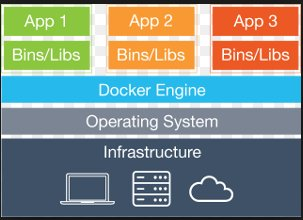
\includegraphics[scale=0.5]{docker.jpg}
\centering
\label{fig:instantaneo}
\end{figure}

A solução proposta por este trabalho, para resolver o problema de associação da evidência a sua origem de modo que o processo seja reprodutível, pausa a execução
do container e coleta um instantâneo da memória dos processos sob sua execução. Este processo é executado em intervalos de tempo conhecidos de modo a se ter uma
evolução da história da memória dos processos. Em um sistema derivado do linux (Ubuntu 14.04) isso foi atingido via cópia do diretório ``\\proc'' relacionado 
aos processos sob o ``cgroup'' associado ao container e salvo em disco. Para relacionar o instantâneo a sua origem, assinamos o arquivo em que salvamos o instantâneo
da memória com o hash da imagem como mostrado na Figura 2.\\

\begin{figure}[h!]
\caption{Evidência salva - hash do container e imagem}
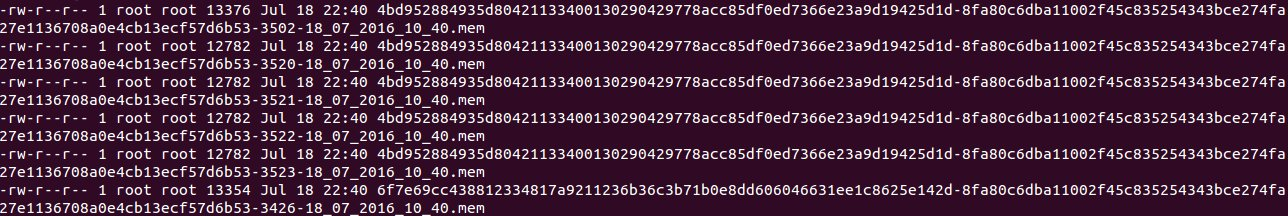
\includegraphics[scale=0.2]{snapshot.jpg}
\centering
\label{fig:instantaneo}
\end{figure}

As técnicas forenses praticadas hoje estão voltadas para a obtenção da informação em sua totalidade, seja via cópia bit a bit, seja por remoção do hardware \cite{Simou2014}
\cite{Bem2008}. Tais práticas tem levado ao crescente volume de dados que os investigadores tem que analisar. Há uma vertente na comunidade chamada ``sniper 
forensics'' onde se coleta e armazena o suficiente para a investigação. A solução proposta por este trabalho acompanha esta tendência, a questão foi definir a quantidade 
de dados ``suficiente'' para uma investigação. De acordo com \cite{Case2014}, detectar intrusões na memória de processos depende de termos uma descrição da memória antes
e depois da intrusão. Com base nisso decidimos que ``suficiente'' seria a quantidade necessária para descrever o sistema antes e depois do ataque. A idéia é 
implementar um log rotativo de instantâneos de memória cobrindo uma quantidade de tempo configurável, integrar a solução com algum sistema de detecção de ameaça de modo
que, ao detectar um ataque, o log passa de rotativo a completo assim permitindo que se conheça o sistema antes e depois do ataque como mostrado na Figura 3. \\

\begin{figure}[h!]
\caption{Janela deslizante de coleta de evidência}
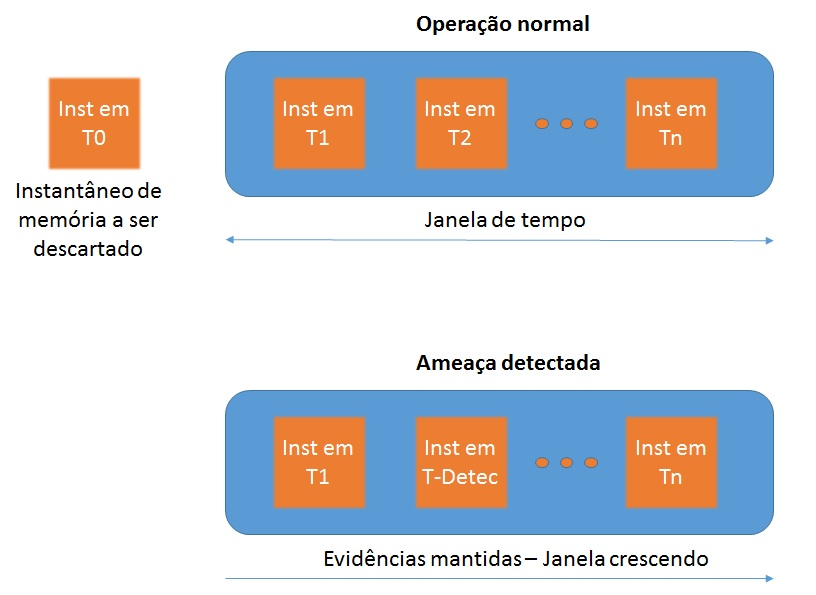
\includegraphics[scale=0.4]{janela.jpg}
\centering
\label{fig:janela}
\end{figure}

De modo a não violar a jurisdição de outros países ou a privacidade de outros usuários por causa do caráter multi-inquilino e multi-jurisdição das arquiteturas em núvem pública,
a solução proposta por este trabalho foi o de armazenar a evidência em um local físico fora da nuvem utilizando como transporte conexão segura. Outro ponto importante é 
garantir a cadeia de custódia da evidência ou seja, garantir que a evidência não foi destruída, alterada ou acessada por qualquer pessoa. Assim a solução proposta por este 
trabalho usará de armazenamento físico fora da nuvem, o transporte será feito por TLS, no momento do armazenamento calcularemos o hash da evidência e o acesso ao mesmo 
será controlado.

Tendo a implementação sido bem sucedida conseguiremos analisar e identificar as formas de ataque enumeradas nos objetivos.\\

\subsection{Implementação}

A implementação da solução foi realizada em um notebook intel I5 de 2.30Mhz e 4Gb de RAM com sistema operacional de 64 bits. Nele, usando Oracle Virtual Box 5.0 criamos uma
máquina virtual com 2 Gb de memória RAM emulando apenas 1 processador.

Na máquina virtual instalamos a versão 1.10 do Docker engine e 1.21 da API, criamos 3 containers, cada um rodando um nginx 1.0 em diferentes portas. Foi escrita uma
aplicação em JAVA que descobre qual o PID associado a cada container e salva o \textbf{/proc/pid/numa\_maps} em um arquivo.

A cópia e gravação do arquivo acontece da seguinte forma, a cada minuto a aplicação pausa o container em questão, tira uma cópia do numa\_maps, salva em um arquivo .mem
e concatenavcom o hash de identificação da imagem. Em seguida verifica qual o arquivo .mem mais antigo em disco, se for mais velho que o tempo 't', o arquivo é descartado.

\subsection{Limitações}

A solução esta focada em coletar informações de memória do user space, ela não enxerga o kernel space. Técnicas de investigação de malware que se baseam em informações
do kernel space como por exemplo a comparação de informações do Process Environment Block (PEB) que ficam no user space com informações do Virtual Address Descriptor (VAD)
que fica no Kernel space não são possíveis. Outro exemplo é a análise de ameaças que realizam manipulação direta dos objetos do kernel ( \textit{D.K.O.M. - Direct Kernel Object Manipulation} )
também não se beneficiam de associação com o container.

A solução completa com todos os elementos descritos anteriormente pode ser visto na figura 4

\begin{figure}[h]
\caption{Solução completa}
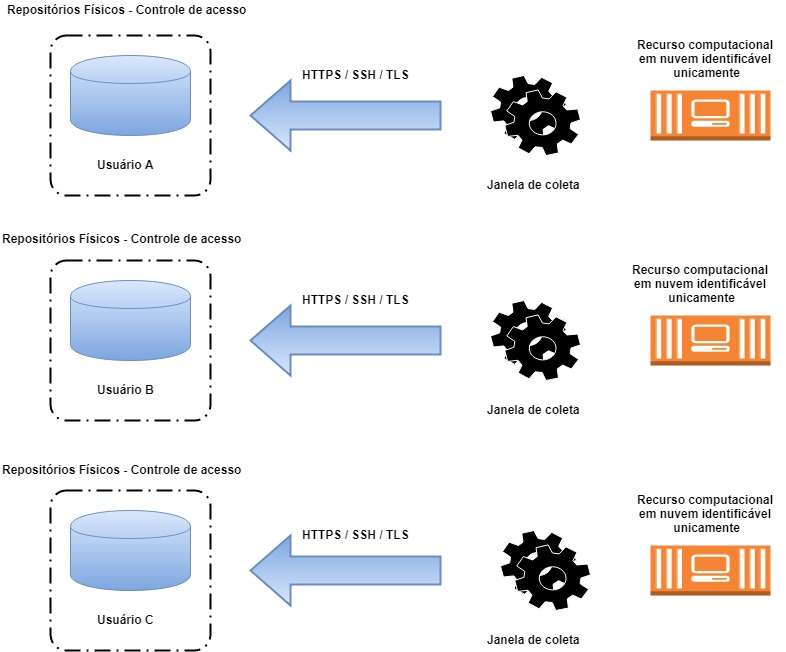
\includegraphics[scale=0.25]{solucao.jpg}
\label{fig:Solucao}
\end{figure}

% An example of a floating figure using the graphicx package.
% Note that \label must occur AFTER (or within) \caption.
% For figures, \caption should occur after the \includegraphics.
% Note that IEEEtran v1.7 and later has special internal code that
% is designed to preserve the operation of \label within \caption
% even when the captionsoff option is in effect. However, because
% of issues like this, it may be the safest practice to put all your
% \label just after \caption rather than within \caption{}.
%
% Reminder: the "draftcls" or "draftclsnofoot", not "draft", class
% option should be used if it is desired that the figures are to be
% displayed while in draft mode.
%
%\begin{figure}[!t]
%\centering
%\includegraphics[width=2.5in]{myfigure}
% where an .eps filename suffix will be assumed under latex, 
% and a .pdf suffix will be assumed for pdflatex; or what has been declared
% via \DeclareGraphicsExtensions.
%\caption{Simulation Results.}
%\label{fig_sim}
%\end{figure}

% Note that IEEE typically puts floats only at the top, even when this
% results in a large percentage of a column being occupied by floats.


% An example of a double column floating figure using two subfigures.
% (The subfig.sty package must be loaded for this to work.)
% The subfigure \label commands are set within each subfloat command,
% and the \label for the overall figure must come after \caption.
% \hfil is used as a separator to get equal spacing.
% Watch out that the combined width of all the subfigures on a 
% line do not exceed the text width or a line break will occur.
%
%\begin{figure*}[!t]
%\centering
%\subfloat[Case I]{\includegraphics[width=2.5in]{box}%
%\label{fig_first_case}}
%\hfil
%\subfloat[Case II]{\includegraphics[width=2.5in]{box}%
%\label{fig_second_case}}
%\caption{Simulation results.}
%\label{fig_sim}
%\end{figure*}
%
% Note that often IEEE papers with subfigures do not employ subfigure
% captions (using the optional argument to \subfloat[]), but instead will
% reference/describe all of them (a), (b), etc., within the main caption.


% An example of a floating table. Note that, for IEEE style tables, the 
% \caption command should come BEFORE the table. Table text will default to
% \footnotesize as IEEE normally uses this smaller font for tables.
% The \label must come after \caption as always.
%
%\begin{table}[!t]
%% increase table row spacing, adjust to taste
%\renewcommand{\arraystretch}{1.3}
% if using array.sty, it might be a good idea to tweak the value of
% \extrarowheight as needed to properly center the text within the cells
%\caption{An Example of a Table}
%\label{table_example}
%\centering
%% Some packages, such as MDW tools, offer better commands for making tables
%% than the plain LaTeX2e tabular which is used here.
%\begin{tabular}{|c||c|}
%\hline
%One & Two\\
%\hline
%Three & Four\\
%\hline
%\end{tabular}
%\end{table}


% Note that IEEE does not put floats in the very first column - or typically
% anywhere on the first page for that matter. Also, in-text middle ("here")
% positioning is not used. Most IEEE journals/conferences use top floats
% exclusively. Note that, LaTeX2e, unlike IEEE journals/conferences, places
% footnotes above bottom floats. This can be corrected via the \fnbelowfloat
% command of the stfloats package.

\section{Trabalhos futuros}

Apesar do sucesso em salvar a memória relacionadas ao container e sua associação com a origem, não foi possível até o momento relizar a análise. As ferramentas de 
leitura de memória disponíveis no mercado até o momento dependem que todo o conteúdo da memória da máquina esteja disponível para realização da análise. Como coletamos 
apenas a memória relacionada aos processos o ferramental não funciona. É necessário um desenvolvimento de uma ferramenta que trabalhe sem a memória completa da máquina,
ou no caso da ferramenta \textit{Volatility} é necessário a criação de um profile para a memória do processo.


% trigger a \newpage just before the given reference
% number - used to balance the columns on the last page
% adjust value as needed - may need to be readjusted if
% the document is modified later
%\IEEEtriggeratref{8}
% The "triggered" command can be changed if desired:
%\IEEEtriggercmd{\enlargethispage{-5in}}

% references section

% can use a bibliography generated by BibTeX as a .bbl file
% BibTeX documentation can be easily obtained at:
% http://www.ctan.org/tex-archive/biblio/bibtex/contrib/doc/
% The IEEEtran BibTeX style support page is at:
% http://www.michaelshell.org/tex/ieeetran/bibtex/
%\bibliographystyle{IEEEtran}
% argument is your BibTeX string definitions and bibliography database(s)
%\bibliography{IEEEabrv,../bib/paper}
%
% <OR> manually copy in the resultant .bbl file
% set second argument of \begin to the number of references
% (used to reserve space for the reference number labels box)
\begin{thebibliography}{1}

\bibitem{Amazon2016}
{AMAZON. \emph{{Amazon Media Room Press Release}}.
[S.l.], 2016. 2~p.}

\bibitem{Bash2015a}
{KEYUN, R. et al. \emph{{Advances in Digital Forensics IV}}. 7. ed. Orlando:
  [s.n.], 2011. 35--46~p.
ISSN 1098-6596.
ISBN 9788578110796.}

\bibitem{Dykstra2012a}
{DYKSTRA, J.; SHERMAN, A.~T. {Acquiring forensic evidence from
  infrastructure-as-a-service cloud computing: Exploring and evaluating tools,
  trust, and techniques}.
\emph{Digital Investigation}, Elsevier Ltd, v.~9, n. SUPPL., p. S90--S98, 2012.
ISSN 17422876.}
  
\bibitem{George2012}
GEORGE, S.; VENTER, H.; THOMAS, F. {Digital Forensic Framework for a Cloud
  Environment. In:  CUNNINGHAM, P.; CUNNINGHAM, M. (Ed.). \emph{IST Africa
  2012}. Tanzania: Internation Information Management Corporation, 2012.
  p.~1--8.
  ISBN 9781905824342.}
  
\bibitem{Poisel2013}
{POISEL, R.; MALZER, E.; TJOA, S. {Evidence and cloud computing: The virtual
  machine introspection approach}.
\emph{Journal of Wireless Mobile Networks, Ubiquitous Computing, and Dependable
  Applications}, v.~4, n.~1, p. 135--152, 2013.
ISSN 20935374 (ISSN).}

\bibitem{Dykstra2013}
{DYKSTRA, J.; SHERMAN, A.~T. {Design and implementation of FROST: Digital
  forensic tools for the OpenStack cloud computing platform}.
\emph{Digital Investigation}, Elsevier Ltd, v.~10, n. SUPPL., p. S87--S95,
  2013.
ISSN 17422876.}

\bibitem{Reichert2015}
{REICHERT, Z.; RICHARDS, K.; YOSHIGOE, K. {Automated forensic data acquisition
  in the cloud}.
\emph{Proceedings - 11th IEEE International Conference on Mobile Ad Hoc and
  Sensor Systems, MASS 2014}, p. 725--730, 2015.}

\bibitem{Sang2013}
{SANG, T. {A log-based approach to make digital forensics easier on cloud
  computing}.
\emph{Proceedings of the 2013 3rd International Conference on Intelligent
  System Design and Engineering Applications, ISDEA 2013}, p. 91--94, 2013.}
  
\bibitem{Dezfouli2012}
{DEZFOULI, F.~N. et al. {Volatile memory acquisition using backup for forensic
  investigation}.
\emph{Proceedings 2012 International Conference on Cyber Security, Cyber
  Warfare and Digital Forensic, CyberSec 2012}, p. 186--189, 2012.}
  
\bibitem{Dolan-Gavitt2011a}
{DOLAN-GAVITT, B. et al. {Virtuoso: Narrowing the semantic gap in virtual
  machine introspection}.
\emph{Proceedings - IEEE Symposium on Security and Privacy}, p. 297--312, 2011.
ISSN 10816011.}

\bibitem{VanBaar2014}
{BAAR, R.~B. van; BEEK, H. M.~A. van; EIJK, E.~J. van. {Digital Forensics as a
  Service: A game changer}.
\emph{Digital Investigation}, Elsevier Ltd, v.~11, p. S54--S62, 2014.
ISSN 17422876.}

\bibitem{Zhang2010}
{ZHANG, L.; ZHANG, D.; WANG, L. {Live Digital Forensics in a Virtual Machine}.
  In:  \emph{2010 Internation Conference on Computer Application and System
  Modelling (ICCASM 2010)}. [S.l.: s.n.], 2010. v.~6, p. 328--332.}
  
\bibitem{Aljaedi2011}
{ALJAEDI, A. et al. {Comparative Analysis of Volatile Memory Forensics}.
\emph{IEEE International Conference on Privacy, Security, Risk and Trust
  (PASSAT) and IEEE International Conference on Social Computing (SocialCom)},
  p. 1253--1258, 2011.}
  
\bibitem{Do2014}
{BARBARA, D. \emph{{Desafios da per{\'{i}}cia forense em um ambiente de
  computa{\c{c}}{\~{a}}o nas nuvens}}.
[S.l.], 2014.}

\bibitem{Simou2014}
{SIMOU, S. et al. {Cloud forensics: Identifying the major issues and
  challenges}.
\emph{Lecture Notes in Computer Science (including subseries Lecture Notes in
  Artificial Intelligence and Lecture Notes in Bioinformatics)}, v. 8484 LNCS,
  p. 271--284, 2014.
ISSN 16113349.}

\bibitem{Bem2008}
{BEM, D. et al. {Computer Forensics - Past , Present and Future}.
\emph{Journal of Information Science and Technology}, v.~5, n.~3, p. 43--59,
  2008.}
  
\bibitem{Case2014}
{CASE, A. et al. \emph{{The Art of Memory Forensics: Detecting malware abd
  threats in Windows, LInux and Mac memory}}. Kindle edi. [S.l.]: Wiley, 2014.}
  
\bibitem{Sousa2009}
{SOUSA, F. R.~C.; MOREIRA, L.~O.; MACHADO, J.~C. {Computa{\c{c}}{\~{a}}o em
  Nuvem: Conceitos, Tecnologias, Aplica{\c{c}}{\~{o}}es e Desafios}.
\emph{II Escola Regional de Computa{\c{c}}{\~{a}}o, Ceara, Maranh{\~{a}}o,
  Piau{\'{i}} (ERCEMAPI)}, v.~1, n. EDUFPI, p. 150--175, 2009.}
  
\bibitem{Charters2008}
{CHARTERS, I.; SMITH, M.; MCKEE, G. {The Evolution of Digital Forensics}. In:
  \emph{Techno Forensics 2008 Conference}. [S.l.: s.n.], 2008. p. 1--39.}

\bibitem{Grispos2012}
{GRISPOS, G.; STORER, T.; GLISSON, W. {Calm before the storm: the challenges of
  cloud computing in digital forensics}.
\emph{International Journal of Digital Crime and Forensics}, v.~4, n.~2, p.
  28--48, 2012.
ISSN 1466640073.}

\bibitem{Sharma2012}
{SHARMA, H.; SABHARWAL, N. {Investigating the Implications of Virtual
  Forensics}.
\emph{Advances in Engineering, Science and Management (ICAESM), 2012
  International Conference on}, p. 617--620, 2012.}
  
\bibitem{Rafique2013}
{RAFIQUE, M.; KHAN, M. N.~A. {Exploring Static and Live Digital Forensics:
  Methods, Practices and Tools}.
\emph{International Journal of Scientific {\&} Engineering Research}, v.~4,
  n.~10, p. 1048--1056, 2013.}
  
\bibitem{Quick2014}
{QUICK, D.; CHOO, K. K.~R. {Impacts of increasing volume of digital forensic
  data: A survey and future research challenges}.
\emph{Digital Investigation}, Elsevier Ltd, v.~11, n.~4, p. 273--294, 2014.
ISSN 17422876.}

\bibitem{Miller2004}
{Miller, M. and Turkulainen, J. {Remote Library Injection}.
\emph{www.nologin.org}, 2004. }

\bibitem{Fewer2008}
{Fewer, Stephen {Reflective DLL Injection}.
\emph{harmonysecurity.com}, 2008. }

\end{thebibliography}

% that's all folks
\end{document}


